\section{Introduction}


 


Question Answering (\abr{qa}) is an \textsc{ai} complete
problem~\cite{webber-92}, but existing \abr{qa} datasets do not rise
to the challenge: they lack key \textsc{nlp} problems like anaphora
resolution, coreference disambiguation, and ellipsis resolution.
The logic needed to answer these types of questions requires deeper
\textsc{nlp} understanding that simulates the context in which humans
naturally answer questions.

Neural techniques question answering have
improved~\cite{devlin2019bert} machine reading
comprehension~\cite[\abr{mrc}]{rajpurkar-16}: computers can take a
single question and extract answers from datasets like Wikipedia.
However, \abr{qa} models struggle to generalize when
questions do not look like the standalone questions systems in training
data: e.g., new genres, languages, or closely-related
tasks~\cite{yogatama2019learning}.

Conversational question answering~\cite[\abr{cqa}]{reddy2018CoQA} is a
generalization that ask \emph{multiple} questions in an
information-seeking dialogs.
Unlike \abr{mrc}, \abr{cqa} requires models to link questions together
to resolve the conversational dependencies between them: each question
needs to be understood in the conversation context.
For example, the question \textit{``What was he like in that episode?''}
cannot be understood without knowing what \textit{``he''} and
\textit{``that episode''} refer to, which can be resolved using the
conversation context.

\begin{figure}[t!]
	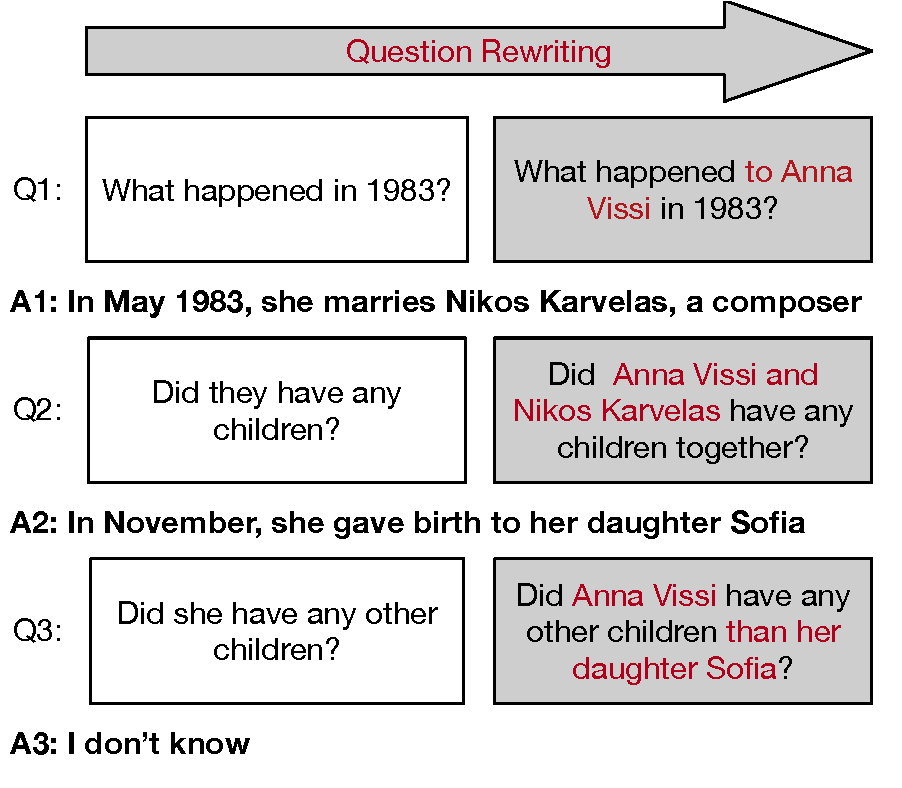
\includegraphics[width=\linewidth]{2019_emnlp_sequentialqa/figures/F1_OmniVersion.pdf}
	\caption{Question-in-context rewriting task. The input to each step
	is a question to rewrite given the dialog history which consists
	of the dialog utterances (questions and answers)  
	produced before the given question is asked. The output is an equivalent, context-independent paraphrase of the input question.}
	\label{fig:example_convo}
\end{figure}

We reduce challenging, interconnected \abr{cqa} examples to
independent, stand-alone \abr{mrc} to create
\name{}---\textbf{C}ontext \textbf{A}bstraction: \textbf{N}ecessary
\textbf{A}dditional \textbf{R}ewritten \textbf{D}iscourse---a new
dataset\footnote{\url{http://canard.qanta.org}} that rewrites
\abr{\quac}~\cite{ChoiQuAC2018} questions.
We crowdsource context-independent paraphrases of \abr{\quac}
questions and use the paraphrases to train and evaluate
question-in-context rewriting.
 



Section~\ref{sec:pp_task} formally defines the task of question
de-contextualization.
Section~\ref{sec:data} constructs \name{}, a new dataset of
question-in-context with corresponding context-independent
paraphrases.
Section~\ref{sec:analysis} analyzes our rewrites (and the underlying
methodology) to understand the linguistic phenomena that make
\abr{cqa} difficult.
We build several baseline rewriting models and compare their
\textsc{bleu} scores to our human rewrites in Section~\ref{sec:expr}.
 